\documentclass[12pt,a4paper,titlepage]{article}


\usepackage[firstinits=false,url=false,isbn=false,style=chicago-authordate,backend=biber,sorting=nyt,maxcitenames=2,uniquelist=false]{biblatex}
\usepackage[margin=1in]{geometry}
\usepackage{graphicx}
\usepackage{setspace}
\renewcommand\labelitemi{}
\title{Is collaboration a good investment? Modeling the link between funds given to collaborative watershed councils and water quality}
%\author{Tyler Scott\\ Evans School of Public Affairs\\University of Washington\\tscott1@uw.edu $|$ 253.632.3362}
%\date{June 2014}

\addbibresource{ScottRef.bib}

\begin{document}

\maketitle

\begin{abstract}


Transboundary problems such as nonpoint source water pollution continue to be a vexing environmental policy challenge. By involving relevant stakeholders in planning, implementation, and management, non-regulatory policy instruments such as collaborative environmental governance seek to increase the comprehensiveness and scale of policy efforts intended to address such problems \parencite{margerum2011}. However, it is unclear whether government funding for collaborative environmental governance efforts pays off in terms of improved environmental outcomes \parencite{thomas2012}. This paper explores a common case of collaborative governance, collaborative watershed councils, specifically examining whether the actions of collaborative watershed councils improve water quality. I couple longitudinal data concerning 2500 state grants given to local watershed councils in the state of Oregon with 20 years of ambient water quality monitoring data sampled at 141 sites around the state. I use state funding as a proxy for watershed council actions, testing whether council actions improve water quality and further comparing the impacts of specific actions such as monitoring, education, administrative support, and restoration. This research presents some of the first evidence about the impacts of collaborative governance that is based upon an objective outcome metric (water quality) \parencite{carr2012,koontz2006}. In modeling these effects, this paper also makes a methodological contribution by demonstrating how spatio-temporal ecological and epidemiological modeling techniques can be used to test policy theory and analyze policy impacts using extant data. Specifically, I use integrated nested Laplace approximation (INLA) \parencite{rue2009} and stochastic partial differential equations (SPDE) \parencite{lindgren2011} to fit a hierarchical Bayesian model that accounts for spatial and temporal dependency. I find that watershed council actions such as education, outreach, and administrative support functions engender strong improvements in water quality. The impacts of restoration actions are positive on average but of lesser magnitude and greater uncertainty.\\

\noindent
\bf{Keywords}: Watersheds, collaborative goverance, non-profits, R-INLA, Bayesian hierarchical modeling
\end{abstract}

\doublespacing

\section*{\bf\MakeUppercase{Introduction}}

Governments increasingly rely on collaborative relationships with non-profit organizations to implement policies or provide services \parencite{salamon2002}. Collaborative management with local nonprofit groups gives governments a community-based vehicle through which to implement policies and programs, and provide nonprofits with access to funding and other resources \parencite{nikolic2008}. Governance arrangements of this form are very common in environmental applications, particularly watershed and water quality management \parencite[e.g.,][]{leach2013,leach2002,margerum2011,hardy2008}. However, while collaborative environmental governance is popular, it is also costly, time-consuming, and subject to considerable uncertainty \parencite{margerum2011}. Thus, the lack of evidence concerning the environmental outcomes of collaborative governance \parencite{thomas2012}, is not just a theoretical gap but a pressing empirical question for public agencies who presumably invest in collaboration with other public, private, and nonprofit stakeholders under the presumption that the benefits will ultimately outweigh the costs. 

In this paper I build on the considerable body of research discussing the role that governments play in--and resultant impacts of--supporting collaborative governance \parencite[e.g.,][]{nikolic2008,lubell2008,ansell2008,emerson2012} by asking a relatively simple question that has proven highly elusive in practice \parencite{koontz2006,carr2012}: Does collaborative governance improve environmental outcomes? To examine this question, I use publicly available water quality monitoring data to explore the impact of 2500 grants given by a state agency, the Oregon Watershed Enhancement Board (OWEB), to local non-profit stakeholder councils engaged in ongoing watershed planning and management activities in watersheds across Oregon over the course of almost 20 years.

To model these data I use Bayesian hierarchical modeling, specifically Integrated Nested Laplace Approximation (INLA) \parencite{rue2009} for estimating complex hierarchical models and Stochastic Partial Differential Equations (SPDE) \parencite{lindgren2011} for modeling spatial and temporal dependency, in order to account for the complex spatio-temporal nature of these data.\footnote{There are of course numerous methodological approaches for modeling spatially and/or temporally correlated observations; in the methodological discussion below, I discuss why I use the SPDE approach and INLA estimation method in particular.} In this paper I also make a methodological contribution to the policy literature by helping to establish the use of these methods for testing public policy and management theory. The INLA approach facilitates large-scale hierarchical models and complex specifications that account for irregular data and spatial and temporal relationships. This enables the use of publicly available, observational environmental data and helps address some of the analytical challenges that have prevented researchers from linking collaborative management efforts to object data concerning environmental outcomes in the past \parencite{koontz2006,thomas2011}.

I use the SPDE-INLA spatial modeling approach to examine whether collaborative watershed council actions (using project-specific funding as a proxy for actions) are associated with measurables change in water quality. Further, I test two broad theoretical hypotheses emerging from the collaborative governance literature. First, I use data on restoration and recovery actions taken by both public agencies and by collaborative watershed councils to examine whether there is a prima facie case that collaborative governance institutions produce more effective outputs (policies, plans, programs, etc.) than do public agencies acting unilaterally. Second, because collaborative governance is often associated with intermediate outcomes such as stakeholder learning and belief change that might enhance the efficacy of future policy and management efforts, I use time series monitoring data and historical grant records to test the relationship between public investment in collaborative governance and the predicted impact of later actions. In what follows, I first describe the theoretical rationale for this research, and then provide background concerning the case analyzed. I then specify my analytical approach and introduce the INLA and SPDE methods. The remaining sections present the data and model results, and discuss the implications of these findings.


\section*{\bf\MakeUppercase{Rationale}}

The idea that policy implementation does not solely involve autonomous actions by public agencies is long-established \parencite[e.g.,][]{ostrom1961} and ubiquitous in modern policymaking \parencite[][p. 8]{salamon2002}. In fact, it is unclear in practice what an alternative to the general concept of collaboration \parencite{donahue2011,agranoff2003}, in which government agencies communicate, consult, coordinate, or cooperate with other public, private, and nonprofit entities, would even be. A stricter definition of collaborative governance, which involves government initiation and/or funding \parencite{ansell2008} for efforts “in which a… group of autonomous stakeholders deliberates to build consensus and develop networks” \parencite[p. 6]{margerum2011} in order to “make or implement public policy or manage public programs or assets” \parencite[p. 544]{ansell2008}, raises a more interesting issue: collaboration by this definition does not just happen, but rather policymakers choose collaborative governance as a means through which to design and implement policies \parencite{layzer2008, hoornbeek2012, koontz2004}. Does using funding nonprofit collaborative stakeholder groups result in improved environmental outcomes? For instance, is it more beneficial for the state of Oregon to implement a restoration project directly or to provide grant funds to a local nonprofit watershed council to implement the restoration project instead?

While collaborative governance is heavily documented in the policy and management literatures \parencite{emerson2012,margerum2011,sabatier2005,ansell2008,lubell2004}, the complexity of social-ecological systems makes it difficult to trace how government support for non-profit collaborative groups ultimately impacts environmental outcomes \parencite{koontz2006, thomas2011}. Clearly, the context of a particular locale or project greatly determines the answer to this question. More broadly, however, the literature concerning collaborative management provides a theoretical basis to help understand the rationale for governments to partner with nonprofit collaborative groups. The general rationale for supporting collaborative management, such as by funding a nonprofit collaborative management group, is that collaborative efforts yield more holistic and comprehensive management. For instance, collaborative management is shown to enhance cooperation amongst stakeholders \parencite{lubell2004}, alter existing stakeholder beliefs \parencite{leach2013}, increase information exchange and learning amongst actors \parencite{beierle2002,weible2009}, foster trust and collective action \parencite{lubell2005}, and incorporate a broader range of information \parencite{innes1999,wondolleck2000}. Local nonprofit collaborative groups can be flexible and responsiveness, pivoting to meet local needs and concerns \parencite{nikolic2008}.

On the other hand, since collaborative management is deliberative and consensus-oriented \parencite{ansell2008}, it can involve a great deal of time and effort \parencite{margerum2011}. Further, in contrast with direct government actions where the implementing agency has stricter control over policy efforts \parencite{salamon2002}, policy implementation via collaborative management has a heightened degree of uncertainty from the perspective of the funding agency since the involvement of more actors creates issues of accountability and control \parencite{weber2003}. There is also concern that government support for local collaborative management efforts can detract from the ability of these local organizations to operate with responsiveness and flexibility, reducing the very qualities that are presumed to make such groups effective \parencite{smith2004,nikolic2008}.

Nonetheless, the use of collaborative management continues to proliferate \parencite{ansell2008,emerson2012} as a response to complex environmental problems \parencite{margerum2011}. Among the practical rationales for public managers to choose collaborative management are the expectations that collaborative management will facilitate a more comprehensive understanding of policy problems \parencite{leach2013}, alleviate conflict between stakeholders \parencite{berardo2014}, reduce interorganizational transaction costs \parencite{emerson2012}, and foster greater “buy-in” from stakeholders \parencite{ansell2008}. In short, policymakers believe that collaborative management will improve the design and implementation of policies and programs and thereby improve policy outcomes.

\section*{\bf\MakeUppercase{Background}}

Nonprofit watershed councils in the state of Oregon have proved to be a fruitful object of study for those interested in collaborative management \parencite{griffin1999,dakins2005,margerum2002,margerum2007,margerum2008,margerum2011,habron2003,margerum2004,hibbard2006, lurie2008}. My study differs significantly from the cited works in that none of these analyses evaluate the water quality impacts of watershed councils on a long-term, statewide basis (most involve intensive case studies that focus on specific watersheds). Created by the state legislature in 1995, OWEB gives grants to local governments, watershed councils, private firms, nonprofit organizations, and local citizens and landowners for restoration and recovery projects and programs. As part of this broader mission, OWEB provides guidance, administrative support, and resources to 87 local watershed councils. This support includes grants to local watershed councils for myriad purposes ranging from environmental assessment to hiring a full-time coordinator. 

Because grants are awarded by OWEB on a competitive basis, these data are not suitable for providing a generalizable estimate of how funding collaborative management in a randomly selected watershed improves water quality. This is because the grant application and approval process is intended to identify and select motivated parties and favorable circumstances, which results in selection bias at the watershed level of analysis. However, what is really of interest in this case is the efficacy of Oregon's statewide support of a collaborative watershed management system. The case that I consider is the state of Oregon’s ongoing financial support for collaborative watershed management. In other words, the purpose of this analysis is to evaluate the statewide OWEB watershed management strategy (of providing public funds to nonprofit management councils) by modeling whether providing funds to watershed councils corresponds to improved water quality. It is difficult to envision a state or regional program not administered on similar grounds (with funds strategically allocated), and thus this analysis thus provides a good conception of the effectiveness of a grant-funded collaborative watershed management system implemented at a regional level.

\section*{\bf\MakeUppercase{Hypotheses}}

OWEB’s statewide, grant-based system also provides a unique way to address one of the challenges typically faced in estimating the impact of collaborative group efforts: even if budget data are available, it is difficult to determine the activities and relative effort level of each group. OWEB grant funds provide a consistent approximation of collaborative management efforts across the state over a many years. Further, funding data provides a continuous metric of council activity that can be used to estimate how increased support for collaborative management relates to environmental outcomes. If collaborative watershed management has an impact on water quality, greater support (as measured by grant funding in this case) should be associated with a larger predicted impact.

\begin{description}
\item{Hypothesis 1 (H1): Grant funds given to nonprofit watershed councils are associated with improved water quality in the target watershed.}
\end{description}

H1 is an important starting place for this analysis, since it addresses the general issue of whether collaborative governance is “all talk and no action” \parencite{lubell2004}. This research is one of the first analyses that is able to leverage objective measures of both collaborative governance actions and environmental outcomes. Thus, establishing an association between watershed council actions and water quality is meaningful in-and-of itself given the dearth of evidence concerning the relationship between collaborative governance and environmental outcomes generally \parencite{carr2012,koontz2006, newig2009}. 

However, from both a theoretical and practical perspective the more important questions concern how watershed council actions compare to public or private environmental policy efforts and the relative impacts of different types of watershed councils actions. Collaboration is time consuming, resource intensive, and uncertain \parencite{margerum2011}, so it is important to consider not just whether collaborative governance efforts improve water quality, but also the efficiency of public investment in collaborative governance. In other words, does collaborative governance achieve better environmental outcomes relative to standard public sector approaches, and are there particularly projects or programs for which collaborative governance is particularly advantageous?

The collaborative governance literature poses two broad rationales as to why investment in collaborative governance can lead to improved environmental outcomes, each of which I use to pose a hypothesis. First, collaborative institutions might simply do a better job. Due to the largely localized nature of--and broader, more diverse stakeholder involvement in--collaborative governance, outputs can be more flexible and context-appropriate \parencite{nikolic2008} as well as better designed and implemented \parencite{sabatier2005}. Further, collaborative governance is theorized to engender principled engagement amongst participants that fosters shared motivation, which in turn enables joint actions which could not be accomplished separately \parencite{emerson2012}. Thus, projects carried out by local collaborative watershed councils might be expected to have a stronger association with improved water quality than projects conducted by local and regional governments. 

Soil and water conservation districts (SWCDs) in Oregon provide a basis for comparison in this regard. SWCDs (in some states known instead as resource conservation districts or natural resource districts) are special districts required by state law to implement natural resource management. In Oregon, the Oregon Department of Agriculture provides services to 45 SWCDs throughout the state; thus, SWCDs are relatively similar in breadth and scope state watershed councils. Both watershed councils and SWCDs are eligible to apply for water quality improvement grants from OWEB. Thus, Hypotheses 2 seeks to compare the predicted impact of water quality improvement funds given to local governments (SWCDs) versus collaborative nonprofit watershed councils: 

\begin{description}
\item{Hypothesis 2 (H2): Grant funds given to nonprofit watershed councils are associated with greater water quality improvements than grants given to local SWCDs.}
\end{description}

Second, collaborative governance efforts can have a capacity building effect. Collaborative governance has been linked to “intermediate outcomes” \parencite{carr2012} such as belief change, social capital, and stakeholder learning \parencite[e.g.,][]{leach2013,gerlak2011,calanni2014}. These intermediate outcomes can improve the efficacy of policies and programs by altering existing incentives and costs \parencite{schneider2003}, for instance by reducing transaction costs or garnering increased support for management actions. 

OWEB invests in such capacity building by providing grants explicitly for council support, funding administrative activities, staffing, and operations. Adequate support in this regard is shown to be critical to for collaborative efforts to be successful \parencite{lubell2009}. In particular, there are significant transaction costs associated with initiating and maintaining inter-organizational endeavors, and government provision of staffing, infrastructure, and other resources are shown to facilitate such network relationships \parencite{schneider2003}. “Program logic” \parencite{bickman1987} is the narrative for how a given program will work to address an identified problem \parencite{margerum2011,mclaughlin1999}. To put a fine point on a broad and nuanced literature, the program logic for investing in council support is that a well-functioning collaborative group will result in policy and program outputs that draw on more relevant perspectives \parencite{ansell2008,oleary2006,leach2006}, have increased commitment from participants \parencite{bryson2006,ansell2008}, and could not be produced separately \parencite{emerson2012}. Based upon this rationale, one would expect that projects and programs carried out in watersheds where there is--or has been--greater investment in capacity building to have a stronger positive association with water quality improvements. 

\begin{description}
\item{Hypothesis 3 (H3): Grant funds given to nonprofit watershed councils are associated with stronger water quality improvements in watersheds where prior capacity building investments have been greater.}
\end{description}



\section*{\bf\MakeUppercase{Model and Methods}}

In accordance with these hypotheses, the goal of this paper is to estimate the association between grants given to watershed councils and subsequent water quality. Water quality index observations ($Y_{itj}$) occur at location $i$ in time period $t$ within stratum (HUC8 watershed in this case) $j$. Standard regression models are inappropriate in this application, since it is expected that two observations near to each other in spatial location or time, or within the same administrative boundary (e.g., under the purview of a given watershed council) are more similar than two randomly selected observations (and thus exhibit residual dependency, i.e., correlated residuals). These data are thus highly similar to many epidemiological data contexts, as there is an outcome (water quality) and a “risk factor” or “confounder” (grant funded projects) and where the spatial (sample sites in the state of Oregon) and temporal (monthly observations) structure of the data must be accounted for in order to make valid inferences. Accordingly, I use a suite of Bayesian hierarchical modeling methods found primarily in the epidemiological \parencite{cameletti2013,blangiardo2010,blangiardo2013}, spatial econometrics \parencite{bivand2008,bivand2013,gomez-rubio2014}, and ecological modeling \parencite{cosandey-godin2014, clark2005,clark2006,wikle2003,cressie2009,wikle2010,xu2007,cressie2011} literatures.

A Bayesian model derives a statistical result (the “posterior distribution”) via an inferential process that combines the “prior distribution” (what was assumed prior to observing additional data) with the current data model \parencite{bernardo2009}. For this application, there are two primary advantages of the Bayesian approach. First, since a posterior parameter distribution is estimated by the model, it is easy to obtain the posterior probability that the parameter does or does not exceed a given value \parencite{blangiardo2013}; this is easier to interpret than p-values used in frequentist statistics. Second, Bayesian methods greatly ease the use of hierarchical model structures, which use random effects to model variance at multiple levels of a model. The Bayesian model I use includes random effects that model spatial and temporal dependence amongst observations. Bayesian methods are shown to be highly effective for analyzing data with this type of spatio-temporal structure \parencite{dunson2001}.

Hierarchical Bayesian models are typically fit using Markov chain Monte Carlo (MCMC) algorithms which use a simulation-based approach to model the posterior parameter distributions \parencite{brooks2011,robert2004,lesage2010}. Since these methods rely on a very large number of simulations applied to complex model structures, MCMC methods are greatly time- and computationally-intensive \parencite{blangiardo2013}. In lieu of MCMC, I use a more computationally efficient method, Integrated Nested Laplace Approximation (INLA), developed by \textcite{rue2009} and widely employed for Bayesian hierarchical modeling \parencite{beguin2012,martino2011,martino2010,lindgren2011,cosandey-godin2014}.

Given that INLA is relatively new and has as-of-yet limited penetration into the policy literature, along with describing the model specification used in this paper I also provide background on the INLA estimation method more generally. A full description of the INLA methodology is beyond the scope of this paper; \textcite{rue2014} and \textcite{lindgren2013} provide excellent technical background. Based on the specifications of \textcite{cameletti2013}and \textcite{cosandey-godin2014} for a spatio-temporal point-reference model, water quality observations in a given watershed at a specific time and location are linked to a structured additive predictor $\eta$ that is defined linearly as:

\begin{equation}
\eta = \alpha_{h[i]} + \sum_{m=1}^{M} \beta_{m}Site_{i} + f(.) + \zeta_{t[i]} + \tau_{t[i]}
\label{eq:obslevel}
\end{equation}

where $\beta_{m}$ is the coefficient associated with site covariate $m$ for observation $i$ (including elevation and distance from coast); $f(.)$ represents the semi-parametric function used to model the spatio-temporal random effect (described in more detail below); $\tau_{t[i]}=(t_1,...,t_T)$ represents a smoothed linear trend (a generalized additive model [GAM] term) accounting for long term water quality trajectory; $\zeta_{t[i]} = (t_1,...,t_T)$ is a seasonal component with periodicity ($p=12$) to account for expected seasonal variation in water quality in Oregon, particularly between low-flow (June to September) and high-flow (October to May) months \parencite{cude2001}; and $\alpha_{h[i]}$ is the random intercept estimated for observation $i$ in a given HUC8 watershed $h$. The advantage of fitting a random group effect as opposed to a fixed effect is twofold. First, the random effect accounts for differing within-group sample sizes by placing more emphasis on the group mean when there are many observations in the group and drawing more broadly from the population mean when there are very few observations in the group \parencite{gelman2006,gelman2013}. This helps ensure that predicted differences between watersheds are not simply a product of small within-watershed sample sizes by attenuating the group-level estimates for watersheds with fewer water quality samples towards the overall mean (producing more conservative group-level estimates than would a basic fixed-effect approach). Second, and of particular importance for this analysis, is that the random group effect can itself be modeled as a function of group-level covariates. This includes important water quality control variables, such as the percentage of land in the watershed that is developed (e.g., paved or contains buildings) and that is used for agricultural purposes. It also includes grant funding, the variable(s) of interest. Since grants are given to watershed councils, it makes the most sense to aggregate funding at the watershed level. The HUC8-specific adjustment is thus itself modeled as:

\begin{equation}
\alpha_{h} = \alpha_{0} + \sum_{w=1}^{W}\gamma_{w}Watershed_{wj[i]}
\label{eq:huc8level}
\end{equation}

where $\alpha_0$ is the population average and $\gamma_w$ represents a vector of coefficients corresponding to watershed-level variables 1 to $W$ for an observation ($i$) in a given watershed ($h$).

INLA facilitates Bayesian inference on model parameters by assuming that these model parameters collectively constitute a latent field, $\theta = \{\alpha_j,\beta_m,f,\zeta_t,\tau_t\}$. This latent field is in turn assumed to be a defined by a Gaussian multivariate distribution of mean 0 and precision matrix $Q(\psi)$, such that $\theta \sim N(0,Q^{-1}(\psi)$ \parencite{blangiardo2013,rue2005,rue2009,cosandey-godin2014}. Using this model, an individual observation $y(s_i,t)$ (at location $s$ and time $t$) is modeled by a subset of $\theta$ according to its spatio-temporal characteristics:

\begin{equation}
y(s_i,t)|\theta,\psi \sim p(y(s_i,t)|\sum_j,A_{ij}\theta_{j},\psi)
\label{eq:spacetime}
\end{equation}

In Equation ~\ref{eq:spacetime}, the observation matrix $A_{ij}$ is where the SPDE method enters in. In order to account for spatial dependence amongst water quality observations, this model includes a random spatial effect known as a Gaussian random field (GRF) \parencite{cosandey-godin2014}. Modeling a continuous spatial process obviously poses a significant, and largely intractable, computational challenge. The SPDE method posed by \textcite{lindgren2011} indexes the continuous GRF as a discrete random process, or a Gaussian Markov random field (GMRF) \parencite{lindgren2013}, by dividing the spatial domain (the state of Oregon in this case) into a “mesh” of triangles \parencite{blangiardo2013}. Essentially, this triangular grid is used to approximate the continuous field. The observation matrix $A$ contains the values of the spatio-temporal random field at the specific times and locations contained in the dataset and uses these values for parameter estimation \parencite{cosandey-godin2014}. Since values are only stored for specific points (triangle vertices in the mesh) (points within a triangle can be estimated by extrapolating between values at neighboring vertices), this provides considerable computational savings. The latent field is thus linked to model likelihood via $A$, such that $\eta^*=A\eta$ \parencite{cosandey-godin2014}:

\begin{equation}
p(y(s_i,t) | \theta,\psi) = \prod_{i=1}^{n} p(y(s_i,t) | \eta^{*},\psi)
\label{eq:spde}
\end{equation}

\noindent
Further details regarding INLA and SPDE methods are provided in the context of the analysis presented below. First, I describe the data used in this model.

\section*{\bf\MakeUppercase{Data}}

\subsection*{Dependent Variable}
The dependent variable of interest, a water quality index score, is obtained from the Oregon Department of Environmental Quality (ODEQ). The Oregon Water Quality Index (OWQI) is a multimetric index that integrates eight water quality variables (temperature, dissolved oxygen, biochemical oxygen demand, pH, total nitrogen, total phosphorus, total solids, and fecal coliform) into one comprehensive metric \parencite{cude2001}. For each of these eight subindices, the analytical measurement is converted into a quality rating between 10 (worst case) and 100 (ideal); ODEQ then uses a harmonic square mean formula:

\begin{equation}
OWQI = \sqrt{\frac{S}{\sum_{s=1}^{S}\frac{1}{SI^{2}_{s}}}}
\label{eq:owqi}
\end{equation}

\noindent
where $SI_s$ refers to subindex $s$ in subindices 1 to $S$ (e.g., pH level), to compute the OWQI score. In this method, the most impaired variable imparts the greatest influence on overall index score \parencite{cude2001}, which thus provides a holistic measure of general water quality (since a site cannot have a relatively high overall score if it performs poorly on any metric). It is important to note that the OWQI is best suited as a comparative metric; not only is the index calibrated specifically for streams in the state of Oregon, but it does not reflect the suitability of water for specific uses (e.g., fishing or swimming). It does, however, provide an excellent synopsis of overall water quality that allows for comparison of observations from across the state over time. In particular, the OWQI is designed to facilitate comparisons between watersheds, and thus sub-indices such as pH and total solids are adjusted to account for geologic variability \parencite{cude2001}.

OWQI scores are observed on an intermittent monthly basis from 1990 to 2013 at 141 monitoring stations. Generally, in the data obtained from ODEQ index scores are tabulated every other month. For instance, some stations have observations in June and August while others have observations in July and September. In a few cases, however, there are only three or four total monthly observations in total at a given site. One major empirical advantage of the INLA hierarchical model and the random effects approach I use is that it can readily handle this type of irregular data. Thus, there is no need to drop any data or to impute data for under-sampled sites or unsampled months. In total, there are 32,908 unique observations occurring between January 1992 and December 2013. 

\subsection*{Independent Variables}

The independent variables of interest are obtained from the Oregon Watershed Enhancement Board (OWEB). The grant database received from OWEB contains record of all grant projects funded by OWEB, including location (watershed), project start and end dates, project type, and funding amount; this analysis specifically considers 3401 grants given to watershed councils and 2329 grants given to SWCDs throughout the state between 1997 and 2013. Table~\ref{table:grantsummary} summarizes the nature of these grants:


% Table created by stargazer v.5.1 by Marek Hlavac, Harvard University. E-mail: hlavac at fas.harvard.edu
% Date and time: Wed, Jul 01, 2015 - 07:39:00 AM
\begin{table}[!htbp] \centering 
  \caption{OWEB grant summary statistics (1997-2013)} 
  \label{table:grantsummary} 
\begin{tabular}{@{\extracolsep{5pt}} ccccc} 
\\[-1.8ex]\hline 
\hline \\[-1.8ex] 
Project & Grantee & N & Average.cost & Average.length..months. \\ 
\hline \\[-1.8ex] 
Capacity & SWCD & $130$ & $109,618$ & $23$ \\ 
 & WC & $401$ & $99,261$ & $27$ \\ 
Outreach & SWCD & $40$ & $24,457$ & $24$ \\ 
 & WC & $189$ & $22,503$ & $18$ \\ 
Restoration & SWCD & $1,890$ & $29,766$ & $26$ \\ 
 & WC & $1,919$ & $58,870$ & $26$ \\ 
Tech & SWCD & $269$ & $41,841$ & $24$ \\ 
 & WC & $688$ & $41,306$ & $26$ \\ 
\hline \\[-1.8ex] 
\end{tabular} 
\end{table} 


While in some cases, a grant is targeted at a specific site (as is often the case for restoration grants), many OWEB grants have a more disparate spatial focus. For instance, an outreach project might be targeted at an entire watershed or basin. To model the spatial focus of grants, grants are aggregated by HUC8 for each month (228 months in total from 1995 to 2013). The total value of a grant is divided by the length of the project in months to calculate a monthly value of each grant; for instance, a \$60,000 grant project started in March, 2001 and ending in May, 2001 results in a value of \$20,000 for each of March, April, and May. While it is unlikely that grant funds are expended uniformly in practice, the “true” model of fund distribution is unclear from these data. The temporal distribution of funds also likely varies greatly between projects in any case. Assuming uniform monthly expenditure across the life of the project provides a consistent approach that is simple to interpret. This method also provides a consistent treatment of projects ongoing as of December, 2013, allocating funds in proportion to the portion of the project timeline that has already passed.

Measuring the impact of grants given to watershed councils poses several significant issues. The causal impact of a grant might not necessarily correspond directly to the actual project period. For instance, a restoration grant used to restore streamside riparian areas should have an ongoing impact on stream turbidity by reducing erosion for years after the project is finished. An OWEB education or outreach grant likewise is expected to have an ongoing impact on stakeholder behavior in the watershed. Of course, in the absence of ongoing maintenance efforts, the effect of restoration or outreach actions likely dissipate or diminish over time. In other words, recording the cumulative total of all grant funding is also inappropriate. To accommodate both the potential for effects that last beyond the actual project duration and for effects that diminish over time, I specify grant funding (for each category of grant) as a rolling sum of active funds for three different time periods: one year, three years, and five years.\footnote{Note that there is a considerable literature speaking to how long it takes for collaborative management efforts to begin to have an impact following inception. For instance, \textcite{leach2002} find that watershed partnerships formed for purposes such as restoration, education, or monitoring often take about 48 months to gain traction. However, what \textcite{leach2002} are in effect referring to is the time it takes for groups to complete projects (particularly how long it takes for a newly formed watershed council to begin to gain traction). In the case of projects funded by OWEB, each grant-funded project has an inception date and a completion date; thus, there is a clear point at which the project, for better, or worse, is finished, and there is no need to apply a temporal lag as would be the case if one were testing the link between watershed council formation and water quality.} For instance, for the five-year metric, active grant funds in a given watershed in January 2005 are the sum of all monthly grant funds in that watershed between January 2000 and January 2005.


\subsection*{Covariates}

One of the advantages of the spatio-temporal model is that accounting for temporal and spatial relationships between observations serves to address many of the factors that affect water quality. For instance, more or less rainfall than is typical in a given year might affect water quality scores by increasing or reducing water levels; grouping observations by time accounts for this sort of variation. Likewise, the HUC8 random effects describe above account for local characteristics that differ across watersheds, such as management institutions or population. Several additional covariates are included in the model, however, in order to address factors that are not accounted for by controlling for the relative location of an observation in space and time.

First, the western portion of Oregon in between the Pacific Ocean and the Cascade Mountains receives much more rainfall than does the eastern portion and has a much different climate. The distance between a given sample site and the coast makes a considerable difference for observations. Thus, the model includes a variable measuring the Euclidean distance between the sample site and the Oregon coast (mapped using geographical data obtained from the Oregon Geospatial Data Library).

Further, land use and land cover are well established as key drivers of water quality \parencite{tong2002,meador2003}. Agricultural land usage is linked to increased water chemical content \parencite{skaggs1994,johnes1997}. Waterways near developed land also demonstrate higher pollution levels \parencite{wang2001} (e.g., cars that leak oil onto pavement, which then washes into streams). To calculate the proportion of each HUC8 watershed that this used for agricultural purpose or that is developed, I use 30-meter by 30-meter raster (pixel image) data from the National Land Cover Database (NLCD). The NLCD includes national land cover data for 1992, 2001, 2006, and 2011. Using ArcGIS, I first produce a binary “True/False” raster for each land cover type (agricultural land [cropland or pasture], wetlands,\footnote{Wetlands are not included in the model specifications below, as wetlands were not found to be a significant model predictor for any fitted model.} forest, and developed land), where each 30-meter by 30-meter pixel is coded as a “1” if that pixel in the comprehensive NLCD raster corresponds to the designated land cover type, and a “0” otherwise. I then use the \textit{sp} \parencite{pebesma2014} and \textit{raster} \parencite{hijmans2014} packages in R to calculate the mean pixel value of all pixels within a 100-meter radius surrounding each sample site for each land cover type. The buffer zone land cover values calculated using the 1992 NLCD are then matched to water quality observations from 1995-2001, the 2001 NLCD data to water quality observations from 2002 to 2005, the 2006 NLCD data to water quality observations from 2006 to 2010, and the 2011 NLCD data to water quality observations from 2010 to 2013. While it would be ideal to have more fine-grained land cover data, perhaps on a yearly or quarterly basis, the NLCD data in this case satisfy the purpose at hand; the absolute values are less important than having a consistent way to account for relative differences in land usage amongst watersheds. In addition to computing 100m buffer values around each site, I also calculate the proportion of total land cover within each HUC8 that is forested, developed, or used for agriculture. These metrics capture broader land-use behaviors in the watershed that might influence water quality. I also use elevation data obtained from the CGIAR Consortium for Spatial Information using the R \textit{raster} package \parencite{hijmans2014} to control for the elevation of the sample site.

\section*{\bf\MakeUppercase{Model Fitting and Selection}}

Before presenting results specifically pertaining to my hypotheses, I describe how I fit these data into the Bayesian hierarchical model and identify the best-fitting specification. All models are estimated using R (R Core Team, 2013) and the INLA package developed by \textcite{rue2009}. As described above, Bayesian models estimation posterior parameter distributions; this implies that each parameter also has a prior distribution. Since there are no “prior data” in this case, prior estimates are specified vaguely using the default recommended INLA settings \parencite{rue2009} and are said to be “non-informative priors” \parencite{gelman2013}. This means that posterior estimates are almost wholly generated in light of the data (i.e., the priors have little effect on the posterior estimates). The spatial mesh used for the SPDE approach is shown in Figure \ref{fig:mesh}:

\begin{figure}[!ht]
\graphicspath{ {`/Users/TScott/Google\space Drive/quinalt/APPAM_2014/'}}
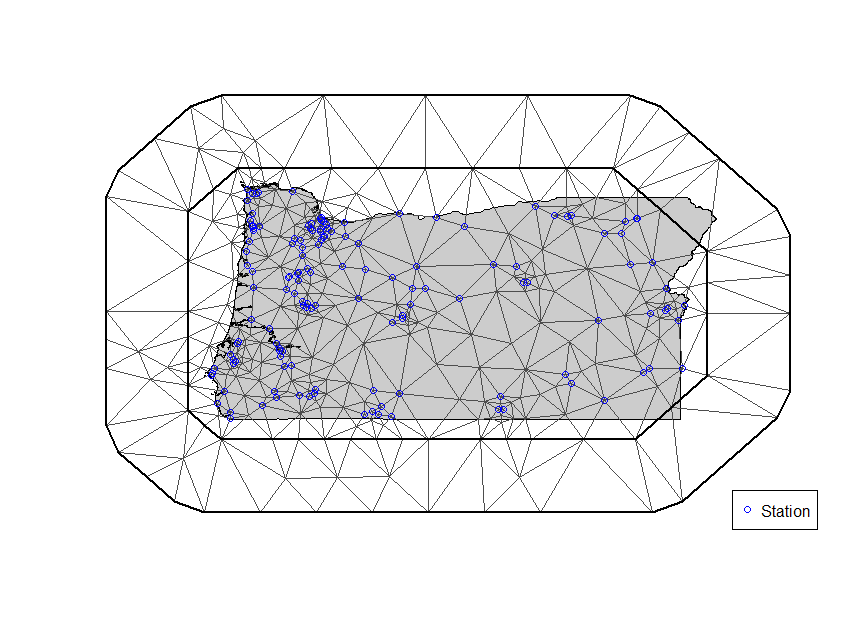
\includegraphics[trim = 30mm 34mm 10mm 30mm, clip, width=6in, height=4in]{oregonmeshplot.png}
\noindent
\caption{\textit{Triangular mesh used for SPDE model}}
\label{fig:mesh}
\end{figure}

Water quality sampling stations can be used, but do not need to be, as triangle vertices in the mesh \parencite{lindgren2011}. The mesh is more finely grained in areas where there are more water quality sampling stations; larger triangles represent areas with little or no information \parencite{cosandey-godin2014}. Essentially, this serves so that the model estimates the field with increased accuracy where there are sufficient data, and conversely does not attempt to model the spatial random effect with great detail where there are no data. This model feature is important, since as Figure \ref{fig:mesh} demonstrates, there fewer water quality sampling stations in much of eastern Oregon. This is due to the fact that there is much less precipitation and fewer streams in the eastern portion of the state. Conversely, the western part of the state is highly concentrated with sample sites, reflecting the much higher density of streams and rivers in this region. Figure \ref{fig:mesh} also shows that the mesh is extended beyond the boundaries of the sample area; this is done to avoid boundary effects wherein there is increased variance at the borders of a spatial field (since locations near the field border have fewer surrounding values) \parencite{lindgren2013}.

There are several possible methods by which to model spatio-temporal correlation, including modeling spatial correlation as constant over time versus fitting a separate spatial correlation structure for each year or month. Temporally changing spatial correlation can for potential changes in the degree of spatial correlation over time (e.g., the location and distribution of fish stocks \parencite{cosandey-godin2014}). For water quality observations, however, one might expect that spatial relationships are more static given that measurement sites are fixed and the distance between sites does not change. Thus, fit a model with spatial correlation being held constant over time. This makes intuitive sense as  “spatial correlation” refers to the underlying spatial process assumed to present; while conditions at different sites might vary considerably, the role that spatial distance plays in these conditions likely remains relatively constant. Table~\ref{table:basemods} presents the results associated with this model as well as a model without an SPDE component (i.e., no spatial correlation) for comparison. Both models contain only covariates and not grant funding data. 


\begin{table}
\caption{Baseline model w/ and w/out spatial correlation}
\begin{center}
\begin{tabular}{l c c }
\hline
                           & w/out spatial correlation & w/ spatial correlation \\
\hline
<<<<<<< HEAD
$\%$  Agric. (100m buffer) & $0.769^{*}$       & $0.938^{*}$       \\
                           & $[0.759;\ 0.780]$ & $[0.915;\ 0.961]$ \\
$\%$  Forest (100m buffer) & $0.912^{*}$       & $1.006$           \\
                           & $[0.897;\ 0.928]$ & $[0.984;\ 1.029]$ \\
$\%$  Devel. (100m buffer) & $0.856^{*}$       & $0.929^{*}$       \\
                           & $[0.843;\ 0.868]$ & $[0.907;\ 0.951]$ \\
$\%$  Devel. in HUC8       & $1.037$           & $0.758^{*}$       \\
                           & $[0.832;\ 1.292]$ & $[0.616;\ 0.932]$ \\
$\%$  Agric. in HUC8       & $0.365^{*}$       & $0.251^{*}$       \\
                           & $[0.270;\ 0.489]$ & $[0.188;\ 0.335]$ \\
$\%$  Forest in HUC8       & $1.080$           & $0.926$           \\
                           & $[0.993;\ 1.175]$ & $[0.853;\ 1.005]$ \\
Elevation (10m)            & $1.038^{*}$       & $0.999$           \\
                           & $[1.034;\ 1.043]$ & $[0.971;\ 1.029]$ \\
Dist. from coast (10km)    & $0.984^{*}$       & $0.994$           \\
                           & $[0.982;\ 0.987]$ & $[0.986;\ 1.002]$ \\
Total Non-OWEB Restoration & $1.014^{*}$       & $1.013^{*}$       \\
                           & $[1.007;\ 1.021]$ & $[1.007;\ 1.019]$ \\
=======
\%  Agric. (1000m buffer) & $0.7678^{*}$        & $0.9337^{*}$        \\
                           & $[0.7566;\ 0.7792]$ & $[0.9101;\ 0.9578]$ \\
\%  Forest (1000m buffer) & $0.9085^{*}$        & $1.0033$            \\
                           & $[0.8927;\ 0.9245]$ & $[0.9808;\ 1.0263]$ \\
\%  Devel. (1000m buffer) & $0.8507^{*}$        & $0.9376^{*}$        \\
                           & $[0.8379;\ 0.8638]$ & $[0.9147;\ 0.9611]$ \\
\%  Devel. in HUC8        & $1.3827^{*}$        & $0.8865$            \\
                           & $[1.1089;\ 1.7235]$ & $[0.7198;\ 1.0915]$ \\
\%  Agric. in HUC8        & $0.4186^{*}$        & $0.2939^{*}$        \\
                           & $[0.3106;\ 0.5596]$ & $[0.2184;\ 0.3954]$ \\
\%  Forest in HUC8        & $1.0717$            & $0.9110^{*}$        \\
                           & $[0.9830;\ 1.1684]$ & $[0.8367;\ 0.9919]$ \\
Elevation (10m)            & $1.0375^{*}$        & $1.0036$            \\
                           & $[1.0333;\ 1.0417]$ & $[0.9741;\ 1.0336]$ \\
Dist. from coast (10km)    & $0.9842^{*}$        & $0.9929$            \\
                           & $[0.9819;\ 0.9864]$ & $[0.9848;\ 1.0013]$ \\
Total Non-OWEB Restoration & $1.0040$            & $1.0057$            \\
                           & $[0.9962;\ 1.0119]$ & $[0.9987;\ 1.0128]$ \\
>>>>>>> 0e5318bd2b0e2c927fc2641854673f1417748195
\hline
DIC                        & 8549.410          & -1832.717         \\
\hline
\multicolumn{3}{l}{\scriptsize{$^* 1$ outside the credible interval}}
\end{tabular}
\label{table:basemods}
\end{center}
\end{table}


As shown in Table~\ref{table:basemods}, the model with spatial correlation performs much better on the Deviance Information Criterion (DIC). DIC is a variation of the traditional Akaike Information Criterion (AIC) score adapted to better suite hierarchical Bayesian models \parencite{ward2008,spiegelhalter2002}. As with AIC (and Bayesian Information Criterion [BIC]) scores, lower DIC scores indicate a better-fitting model. The baseline models also includes terms to capture temporal trends and seasonal fluctuation. Figure~\ref{figure:timetrend} shows the smoothed time trend and seasonal trend fitted as part of Model 3. It is interesting to note that overall, water quality appears to fluctuate between 1992 and 2013 but there is no discernible upward or downward trend.

\begin{figure}[!ht]
\graphicspath{ {`/Users/TScott/Google\space Drive/quinalt/APPAM_2014/'}}
\noindent
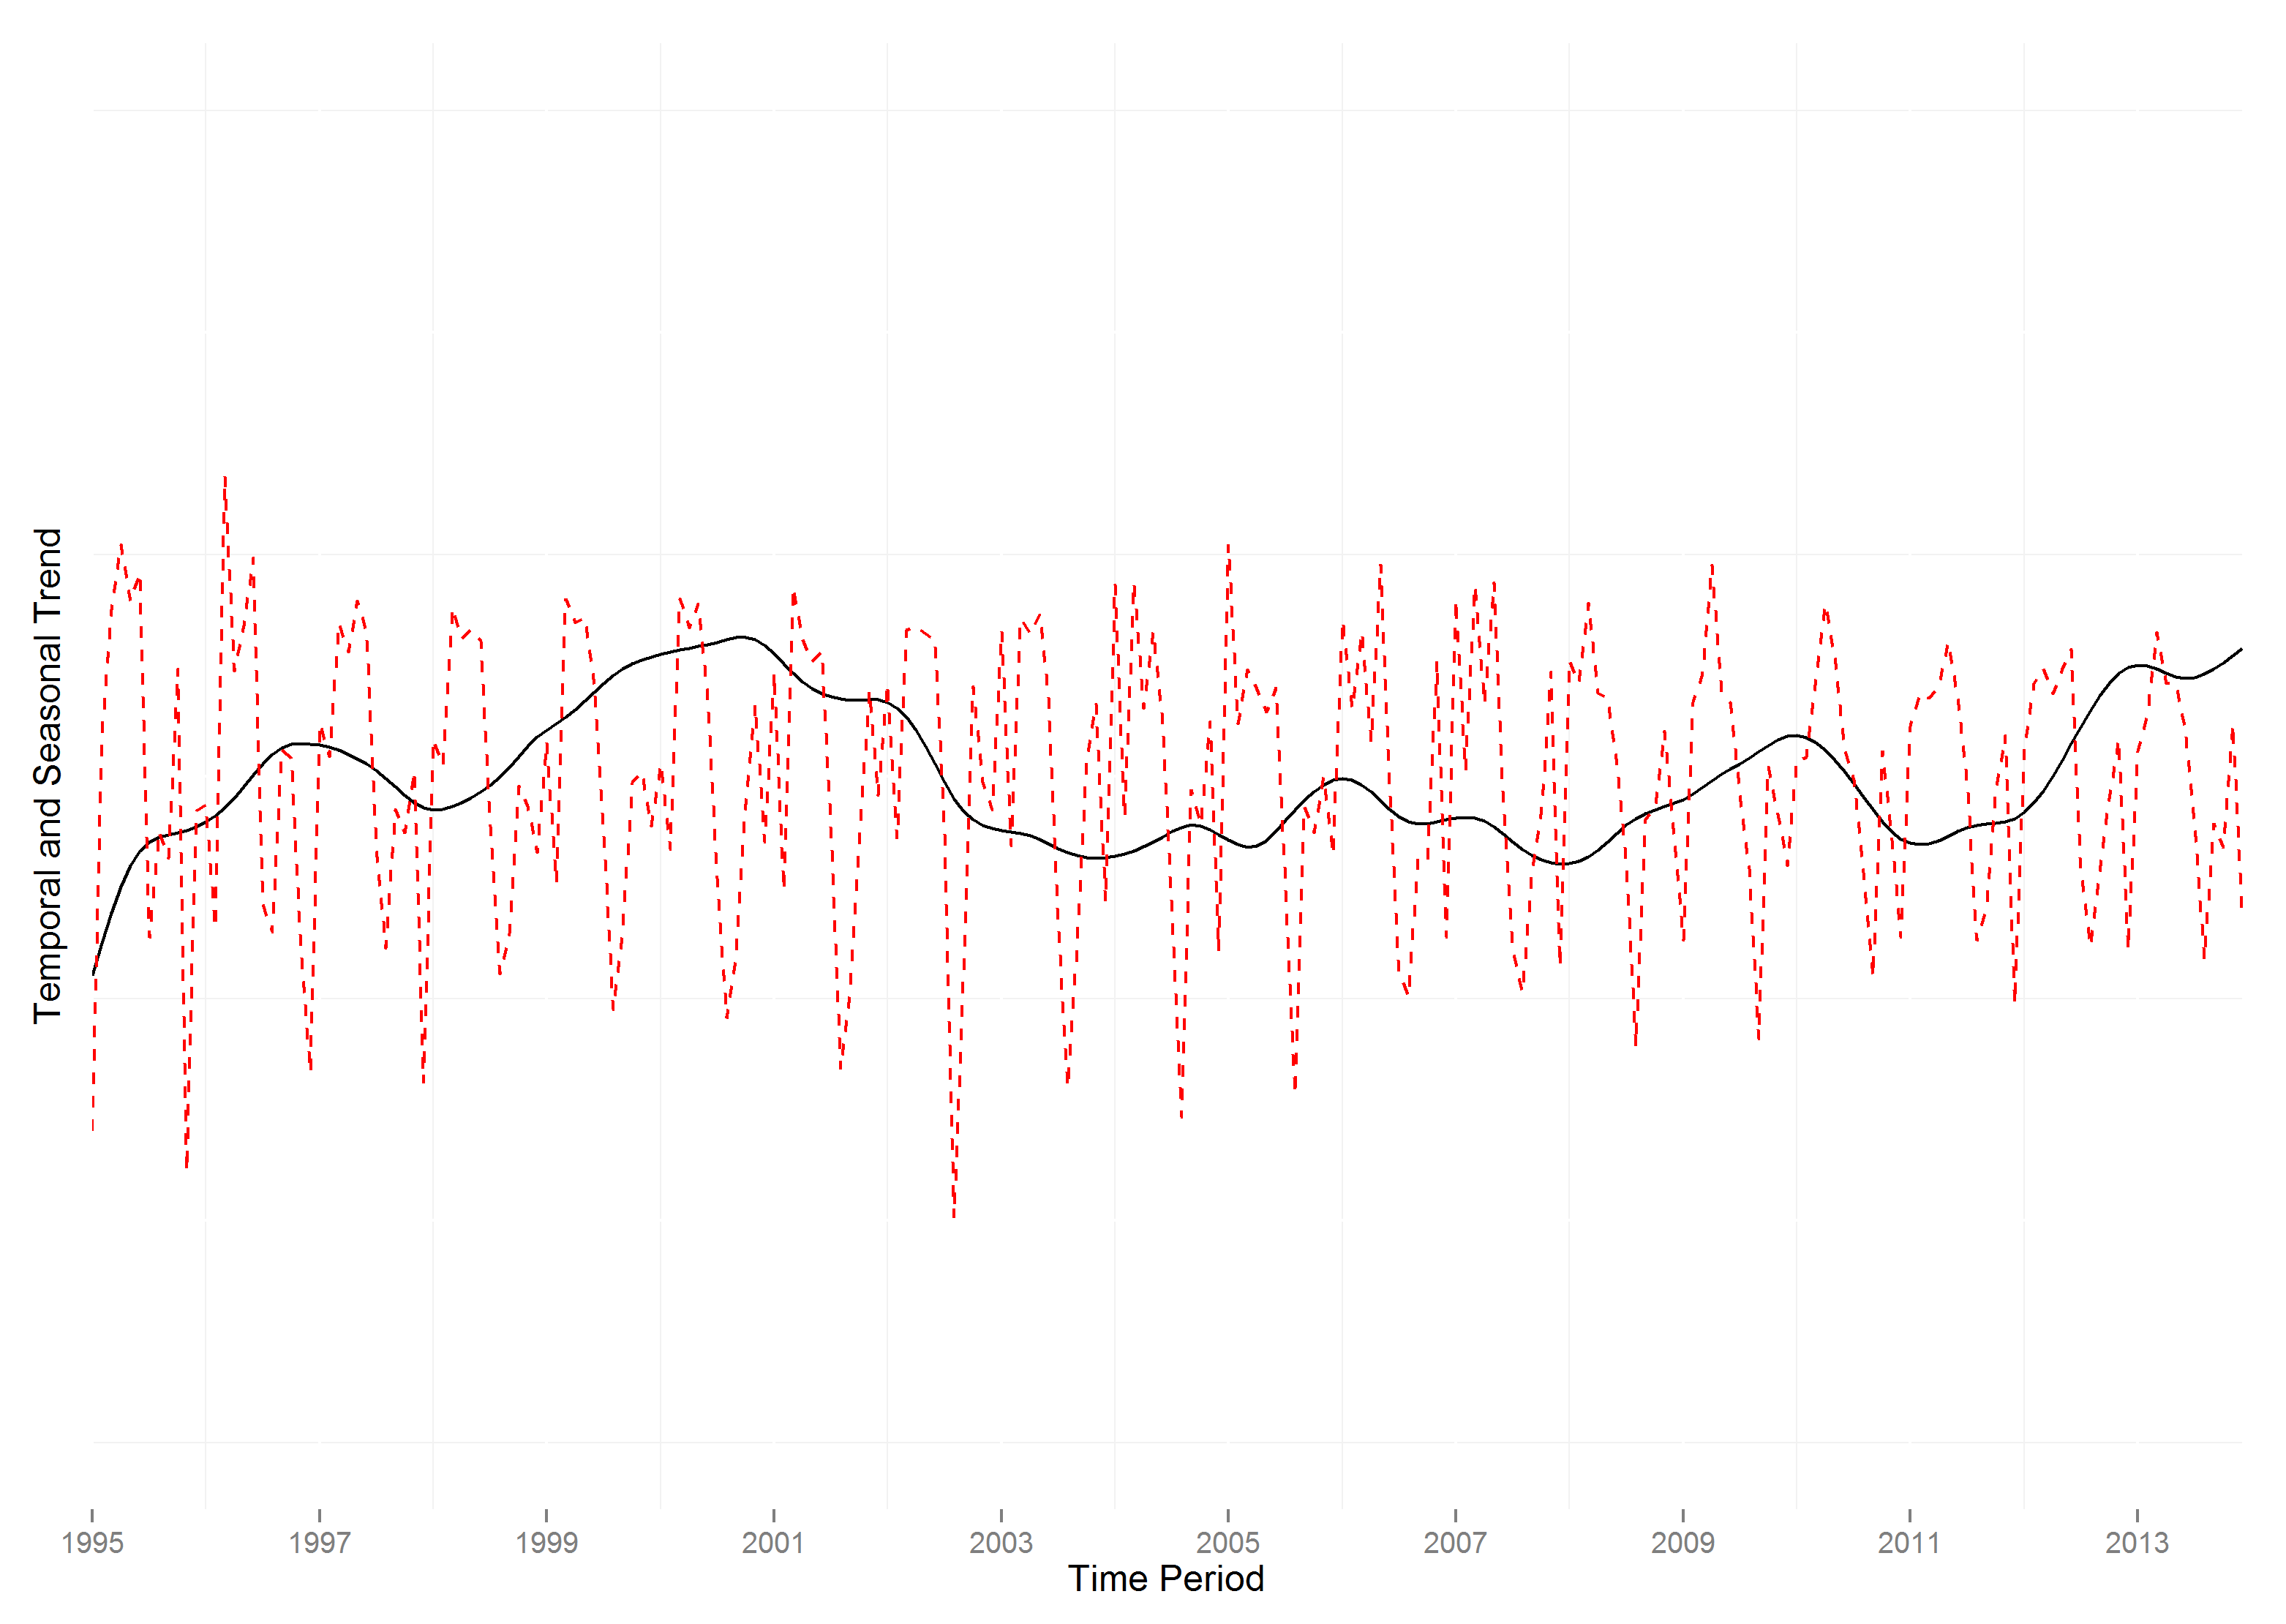
\includegraphics[trim = 4mm 3mm 5mm 18mm, clip, width=6in, height=3.5in]{timetrendplot.png}
\caption{\textit{Smoothed temporal trend and seasonality terms}}
\label{fig:timetrend}
\end{figure}

One other issue that the reader might notice when comparing the coefficient estimates shown in Table~\ref{table:basemods} is that coefficients for the model incorporating spatially correlated errors are in many cases of lesser magnitude. 







Having identified the spatio-temporal correlation structure that best fits these data, I now proceed to fit grant funding into the model. First, I model the predicted impact of all grant funds, regardless of type, computed using rolling 1-year, 3-year, and 5-year sums (e.g., where the 3-year sum represents the total grant funds provided in a given watershed for the 36 months prior to the water quality observation). I use the 1-year interval because water quality is typically considered in terms of a 12-month ``water year,'' and the 3-year and 5-year intervals to potentially capture project impacts realized on a more long term basis. While as mentioned above there are few data that explicitly concern the effects of collaborative management on water quality, \textcite[][p. 281]{lubell2009} note that the perceived effectiveness of collaborative efforts increases with time \parencite[see also][]{leach2002, leach2006}

Table~\ref{table:basecoefs} shows the results of each of these three models. Since the dependent variable, the Oregon WQI score, is log-transformed, each coefficient from the model is interpreted as $log(OWQI) =\alpha+\beta x$, so that a one unit increase in $x$ changes $log(OWQI)$ by $\beta$. An easier way to interpret these coefficients then is to exponentiate each coefficient so that it can be interpreted directly in terms of OWQI score where OWQI increases by a factor of $\exp^{\beta}$. This multiplicative coefficient is how terms in Table~\ref{table:basecoefs} are presented; a coefficient greater than one indicates an increase in OWQI score, and a coefficient less than one indicates a decrease in OWQI score. As described in previously, Bayesian models produce estimates of the posterior distribution for each parameter; thus, what Table~\ref{table:basecoefs} presents is the quantile values that encompass 95\% of the posterior distribution for each parameter. This “credible interval” \parencite{gelman2013} is somewhat analogous to the confidence interval derived from a Frequentist approach; since the exponentiated coefficients are interpreted multiplicatively, the primary concern is whether these quantile bounds span 1 (because when $\beta=1$, $x*\beta=x$, indicating no predicted impact). Bounds that do not span one indicate a “significant” parameter, i.e., one that is statistically unlikely to be equal to zero. The DIC scores for each model in Table~\ref{table:basecoefs} are very similar, as is expected given the similarity between the 1-year, 3-year, and 5-year metrics; each model has a lower DIC score than Model 3 above, evidencing that the addition of grant funding does improve model fit. Note that each model in Table~\ref{table:basecoefs} also includes an intercept and random effect terms for HUC8 watershed, time, season, and space.\footnote{I use the term ``random effect’’ in the more modern sense where the model takes advantage of the mathematical form of a random effect but (unlike in the traditional usage of the term): (a) does not assume that levels of a random effect are draws from a population; nor (b) am I interested in the larger population from which the random effects are ``sample’’ \parencite[see][]{hodges2014}. \textcite{hodges2014} describes ``new style’’ random effects as formal smoothing devices; for instance, in my model the random effect modeled for each HUC8 watershed smoothes each HUC8 intercept estimate between the completely pooled (i.e., no HUC8 term) and fully non-pooled (i.e., a fixed HUC8 effect) alternatives based upon the sample size and variance observed within each HUC8 group \parencite[see][]{gelman2007}.}. 


\begin{table}
\caption{Statistical models}
\begin{center}
\begin{tabular}{l c c c }
\hline
                                                & Past 12 months & Past 36 months & Past 60 months \\
\hline
<<<<<<< HEAD
OWEB grants to WC ($100k)                       & $1.000^{*}$       & $1.000^{*}$       & $1.000^{*}$       \\
                                                & $[1.000;\ 1.000]$ & $[1.000;\ 1.000]$ & $[1.000;\ 1.000]$ \\
OWEB grants SWCD ($100k)                        & $1.000$           & $1.000$           & $1.000^{*}$       \\
                                                & $[1.000;\ 1.000]$ & $[1.000;\ 1.000]$ & $[1.000;\ 1.000]$ \\
OWEB grants to WC * OWEB grants to SWCD ($100k) & $1.000^{*}$       & $1.000^{*}$       & $1.000^{*}$       \\
                                                & $[1.000;\ 1.000]$ & $[1.000;\ 1.000]$ & $[1.000;\ 1.000]$ \\
=======
OWEB grants to WC (\$100k)                       & $0.9999^{*}$        & $0.9999^{*}$        & $1.0000^{*}$        \\
                                                  & $[0.9998;\ 1.0000]$ & $[0.9999;\ 1.0000]$ & $[0.9999;\ 1.0000]$ \\
OWEB grants SWCD (\$100k)                        & $1.0001$            & $1.0000$            & $1.0000$            \\
                                                  & $[1.0000;\ 1.0003]$ & $[0.9999;\ 1.0000]$ & $[1.0000;\ 1.0000]$ \\
OWEB grants to WC * OWEB grants to SWCD (\$100k) & $1.0000$            & $1.0000^{*}$        & $1.0000$            \\
                                                  & $[1.0000;\ 1.0000]$ & $[1.0000;\ 1.0000]$ & $[1.0000;\ 1.0000]$ \\
>>>>>>> 0e5318bd2b0e2c927fc2641854673f1417748195
\hline
DIC                                             & -1863.647         & -1846.064         & -1843.835         \\
\hline
\multicolumn{4}{l}{\scriptsize{$^* 1$ outside the credible interval}}
\end{tabular}
\label{table:allfunding}
\end{center}
\end{table}


One important issue to note with regards to Table~\ref{table:basemods} is that, as the reader will recognize, the predicted effects of even well-known influencers of water quality such as agricultural land usage are minimal. Similarly, while elevation and distance from the Pacific Ocean are expected to be highly predictive of water quality, these coefficients are shown to be unimportant in this model. The reason for this is that when one controls for spatial correlation, as in the SPDE model, spatial correlation is not a phenomenon in and of itself, but rather is a proxy for covariates that vary geographically such as elevation or land usage. Thus, these fixed effects are blurred out due to``spatial confounding'' \parencite{hodges2014}. Likewise, fitting a smoothed temporal term accounts not only long term climatic and environmental changes, but also for social, political, and economic changes that might otherwise be represented by time-varying covariates such as land usage. Simple hierarchical models, particularly fit without the SPDE method, show each of these covariates to be highly influential for water quality and of an expected sign (i.e., development and agriculture are negatively linked to water quality, forest and elevation are positively linked to water quality). It is interesting to note that developed land is negatively linked to water quality in the non-spatial model, but positively linked to water quality once spatial correlation is factored in, though why this is the case is unclear. Regardless of covariate behavior, the models that account for spatial correlation explicitly are the best predictive models (as shown by comparing Models 1 through 7 with Model 0 in Table~\ref{table:dicscores}).

The implication of this issue is that controlling for spatial correlation makes it very difficult to tease out the impact of any variable that is itself spatially distributed. This includes not only the covariates discussed above, but also grant funds that are distributed to particular watersheds and not others. In light of this, it is noteworthy that Table~\ref{table:basecoefs} does show that increased grant funding is predictive of improved water quality. This association is strongest for grant funds expended in the 12 months prior to the sample, where the middle 95\% of the posterior distribution is between 1.001 and 1.008. In other words, net of all other terms in the model, a \$100,000 in grant funds received in the past year predicts a 0.1\% to 0.8\% increase in water quality index score. This supports Hypothesis 1, that providing increased grant funding to collaborative watershed councils will be associated with improvements in water quality. While magnitude of this change might seem very small at first glance, given: (a) the complexity of factors that influence water quality; and (b) the indirect linkages between grant-funded projects and conditions at sample observation sites, it is noteworthy that the model identifies this relationship.

The terms associated with 3 years and 5 years of prior grant receipts are also positive, but the posterior distribution spans $1.000$. This speaks to the question raised in the data and modeling section concerning the temporal impact of grant projects. 

Table~\ref{table:basecoefs} indicates that the predicted impact of grant funds (considering all grants in total) are most pronounced within 12 months of expenditure, and dissipate somewhat over time. It is important to note that this does not necessarily mean that projects have only a short term impact, but rather likely speaks the complexity of measuring environmental policy impacts more generally: the further in time an observation is from a given policy action, the more difficult it is to disentangle policy impacts from ecological trends and other drivers. I continue to explore the temporal nature of grant funds in the context of specific grant types below. I break down grant funds into four categories: restoration, scientific and technical (grants labeled by OWEB as assessment, monitoring, or technical assistance), and outreach (grants labeled by OWEB as either an outreach or an educational project), and capacity building (grants given by OWEB to support watershed council or SWCD operations). 

Given that OWEB funds are allocated competitively, it is unsurprising that different grant types are somewhat correlated. A more substantive concern, however, is that OWEB uses different grant types as substitutes or else allocates specific grants in conjunction or succession; to the extent that activities sponsored by different grant types are not truly targeting different aspects of the problem but rather are aimed at the same things, comparing different council actions becomes more problematic. To examine this correlation between grant types, I tested numerous interaction specifications, including all two-way interaction terms and a full four-way interaction term (interacting the current funding levels for all four grant types). All interaction terms were negligible, and the non-interaction coefficients varied minimally across the different specifications. This indicates that interaction amongst grant types is not a significant concern in this case, and that the predicted impacts of different council actions (using grant type as a proxy for action) can be viably compared. Table~\ref{table:diffgrants} presents the results for the model with the full four-way interaction terms. 

Table~\ref{table:diffgrants} shows that the mean parameter value for each type of grant funding is positive, indicating (as expected) that grant funds of all kinds improve the impacts of watershed councils. For the 12-month rolling sum, all grants but restoration grants have a posterior parameter distribution for which the middle 95\% of the distribution does not encompass 1.000 (again bearing in mind that since water quality is log-transformed, each coefficient is exponentiated and interpreted as a multiplicative factor). A \$100k increase in education and outreach grant funding within 12 months prior to the water quality observation predicts a 8.4\% increase in water quality at the mean parameter value; scientific and technical support is associated with a 2.2\% increase in water quality, while council administrative support predicts a 2.9\% increase.


% Table created by stargazer v.5.1 by Marek Hlavac, Harvard University. E-mail: hlavac at fas.harvard.edu
% Date and time: Sat, Jan 10, 2015 - 13:10:21
\begin{table}[!hbtp] \centering 
  \caption{Comparing Grant Effects by Type} 

\begin{tabular}{@{\extracolsep{5pt}} cccc} 
\\[-1.8ex]\hline 
\hline \\[-1.8ex] 
 Grant (\$100k) & $\hat{\beta_{12m}} (0.025,0.975)$ & $\hat{\beta_{36m}} (0.025,0.975)$ & $\hat{\beta_{60m}} (0.025,0.975) $\\ 
\hline \\[-1.8ex] 
Restoration & 1.003 (1.000, 1.006) & 1.001 (1.000, 1.002) & 1.001 (1.000, 1.002) \\ 
Ed./Outreach  & 1.084 (1.043, 1.126) & 1.038 (1.023, 1.054) & 1.028 (1.017, 1.038) \\ 
Scientific/Tech.  & 1.022 (1.008, 1.035) & 1.011 (1.005, 1.017) & 1.008 (1.004, 1.012) \\ 
Council Support & 1.029 (1.013, 1.046) & 1.011 (1.005, 1.017) & 1.007 (1.003, 1.011) \\ 
Interaction  & 0.995 (0.991, 1.000) & 1.000 (1.000, 1.000) & 1.000 (1.000, 1.000) \\ 
\hline \\[-1.8ex] 
  \label{table:diffgrants} 
\end{tabular} 
\end{table} 


Using the 36-month rolling sum as a measure of grant funds, all three non-restoration grant types again have posterior distributions where the middle 95\% does not include 1.000. A \$100k increase in education and outreach funding predicts on average a 3.8\% improvement, a \$100k increase in scientific and technical support or in council support both predict a 1.1\% increase. The results for 60-month grant totals are similar, with a \$100k increase in education/outreach, scientific/technical, or council support associated with water quality improvements of 2.8\%, 0.8\%, and 0.7\%, respectively. In the section below, I discuss the implications of these results. Note that for the 12-month grant totals, the interaction term suggests that having multiple types of grants active at the same time slightly reduces the overall predicted impact of grant funding on water quality (by about 0.5\% per \$100k). However, the interaction terms at the 36-month and 60-month totals have both mean estimates and posterior bounds that round to 1.000, indicating that there is little-to-no differential impact associated with having multiple types of grants active over longer periods of time.

\section*{\bf\MakeUppercase{Discussion and Conclusion}}

Table~\ref{table:diffgrants} reveals an interesting pattern: the coefficient means decrease in magnitude (or in two cases remain constant) as the time window for which grants are summed increases, but the posterior distributions become more leptokurtic (i.e., narrower). In other words, as the time window increases, the environmental impact of all grants are estimated to be positive with greater certainty, but the average impact is estimated to lessen. One likely reason for the reduced uncertainty regarding estimated impacts is that the increased time window provides a more consistent measure of ongoing council efforts. These data assume a uniform monthly expenditure profile for the life of every grant type. In practice, different projects (even within a single grant type) certainly have different implementation and output profiles, both during and after the project period. Thus, 36-month and 60-month post expenditure time windows likely best capture all grant expenditures at ``full strength'' (i.e., we can be more certain that each project has run its course), explaining the narrower posterior distributions. The reason why the mean estimates decrease as the time window increases in Table~\ref{table:diffgrants} (and also in Table~\ref{table:basecoefs} for all grants combined) is likely due to the data and measurement approach I employ. Water quality is a product of myriad complex factors, and so it follows that the magnitude of any predicted grant impact should decrease over time simply because there is greater opportunity for intervening factors. While it is possible that the impacts of certain projects do not diminish (or perhaps even increase) over time, from a simple cause-and-effect standpoint the 36-month and 60-month time windows place greater emphasis on projects much more distant to the actual water quality observation.

Measurement challenges also likely account for the fact that I do not identify a significant measurable impact from spending on restoration projects, in spite of the preponderance of ecological and environmental science demonstrating that restoration grants have an environmental impact to one extent or another (assuming the project is conducted). These data were not originally intended to serve the purpose of program evaluation. To best evaluate the efficacy of a grant, one would need to follow up directly with an evaluation protocol that explicitly monitors the outputs of grant-funded projects. However, such data collection efforts would obviously be very costly and time-intensive; OWEB is not able to track impacts in such detail or using comprehensive metrics that allow for comparison across the state. In lieu of direct evaluation data, I use existing Oregon water quality sampling stations, which are selected independently of project sites. This best explains why I find the reverse of what I hypothesize in Hypothesis 2 and do not find a measurable impact from restoration grants. Identifying a measurable impact from restoration projects is particularly challenging in this case because I am essentially selecting a stream point within an HUC8 watershed at random and testing whether spending on restoration projects within that same watershed is associated with water quality at that site. If the sample site is near to the actual restoration project site, then the impact might be clear; if the sample site is nowhere near the project site, then measuring the impact is highly unlikely.

Conversely, these data are likely better suited for evaluating non-restoration projects, since the nonpoint nature of many of these projects (in that restoration occurs at a specific site, whereas an outreach project for instance attempts to influence stakeholder behavior at many sites in the watershed) means the project impact has a broader spatial distribution in practice. For instance, an outreach project might influence various individuals throughout the watershed, and funds supporting council operations might be used to provide tools and services that serve people and organizations throughout the watershed. A randomly selected water quality sample site might be more likely to be nearby a “project site” in this case because there are presumably more ``sites'' involved. Generally speaking, the sampling approach of the OWQI lends itself towards evaluating broader management efforts, not wholesale changes in specific areas. In fact, the OWQI itself is billed explicitly as a tool for evaluating water quality management effectiveness \parencite{cude2001}. While the impact of a restoration project might be very pronounced at or near the project site, these impacts are the most difficult to assess using this model. Thus, while this analysis does support the idea that watershed council actions have a meaningful impact on water quality, it is important to emphasize that these results should not discredit the impact of restoration activities.

The primary implication of these findings are that government investment in collaborative management efforts, specifically providing funds to nonprofit watershed councils in this case, is associated with improvement can produce changes in environmental outcomes. Returning to the investment perspective advanced above, I find that OWEB’s investment in the production of non-environmental outputs (e.g., educational programs, stakeholder meetings, monitoring and data collection) does appears to engender an environmental return. The extant literature described in this paper provides a great deal of theoretical support as to why governments might invest in local nonprofit collaborative management groups. As evidenced by the considerable funding governments provide to collaborative management bodies \parencite[e.g.,][]{sabatier2005}, many practitioners already assume the viability of this type of governance approach. These data provide some of the first available evidence quantifying such returns.

More broadly, this research demonstrates the use of hierarchical Bayesian spatio-temporal modeling as a means by which publicly available observational data produced by states and the Federal government for environmental monitoring purposes can be repurposed to test environmental policy theory and evaluate public environmental programs. While the results of this analysis speak to the tradeoffs amongst different types of environmental projects, the exploratory nature of this work is insufficient to provide direct guidance to policy makers about how they should best allocate limited resources. Nonetheless, this provides a basis for further inquiry. In particular, this analysis advances beyond the limiting ``collaborative'' versus ``non-collaborative'' dichotomy to examine a more interesting and relevant question: how should policymakers distribute resources between policies and programs that produce environmental outputs at a relatively fixed input-output ratio (e.g., restoration projects) and those that produce non-environmental outputs (e.g., meetings, educational programs, administrative support) with the potential for returns that exceed inputs (e.g., motivating landowners and resource users to take restorative actions or modify their environmental behaviors in ways that far outstrip the input level of the original outreach program)? Much additional work is needed to understand how these different types of policies ultimately relate to environmental outcomes.

\section*{Acknowledgments}

An earlier version of this manuscript was presented at the 2014 Association for Public Policy and Management Fall Research Conference in Albuquerque, NM. I thank the participants in this event for their valuable feedback. I also thank Craig Thomas, Ryan Scott, Grant Blume, and Ann Bostrom for feedback on this paper, and three anonymous reviewers for their careful and constructive reviews. I am also greatly indebted to several individuals at the Oregon Watershed Enhancement Board, the Water Quality Monitoring Section within the Oregon Department of Environmental Quality’s (ODEQ) Laboratory and Environmental Assessment Program, ODEQ’S Environmental Solutions Division, and the Network of Oregon Watershed Councils for helping to provide the data that made this work possible. Partial support for this research came from a Eunice Kennedy Shriver National Institute of Child Health and Human Development research infrastructure grant, R24 HD042828, to the Center for Studies in Demography \& Ecology at the University of Washington. All data and code used for this analysis are available by request. 

\printbibliography

\end{document}

